\documentclass{article}

%%% SOME USEFUL PACKAGES %%%
\usepackage[english]{babel} % hyphenation
\usepackage[margin=1.5cm]{geometry} % margins
\usepackage{graphicx} % support for graphics
\usepackage{amsmath} % support for math­e­mat­i­cal typesetting
\usepackage{amssymb} % math­e­mat­i­cal symbols
\usepackage{color} % support for colors
\usepackage{mathtools} % more math­e­mat­i­cal type­set­ting
\usepackage{amsthm} % for defining theorem-like environments
\usepackage{enumerate} % change appearance of numbered lists
\usepackage{framed} % textboxes
\usepackage[format=plain,labelfont=bf,up]{caption} % cus­tomise cap­tions for fig­ures and ta­bles
\usepackage[colorlinks=true,linkcolor=black,urlcolor=blue,linktoc=all, citecolor=black]{hyperref} % hyperlinks
\usepackage{setspace}
\usepackage{verbatim}

%%% CUSTOM COMMANDS %%%
\def\ci{\perp\!\!\!\perp} % statistical independence symbol
\newcommand{\ind}{1\hspace{-2.1mm}{1}} % indicator function
\newcommand{\rl}{\mathbb{R}} % real numbers
\newcommand{\ex}[1]{\mathbb{E} \left\{ #1 \right\}} % expectation operator
\newcommand{\pr}[1]{\mathbb{P} \left\{ #1 \right\}} % probability
\newcommand{\var}[1]{\mathbb{V}\text{ar} \left\{ #1 \right\}} % variance
\newcommand{\cov}[1]{\mathbb{C}{ov} \left\{ #1 \right\}} % covariance
\newcommand{\corr}[1]{\mathbb{C}{orr} \left\{ #1 \right\}} % correlation

\begin{document}
	\title{OSM Lab 2017: DSGE Pset }
	\author{Wei Han Chia}
	\date{Due: 28 July 2017}
	\maketitle
	
	\section*{DSGE}
	
	\subsection*{Exercise 1}
	Consider the Brock and Mirman model characterized by the Euler Equation
	\[ \frac{1}{e^{z_t} K_t^{\alpha} - K_{t+1}} = \beta \mathbb{E}_t \left( \frac{\alpha e^{z_{t+1}} K_{t+1}^{\alpha -1}}{e^{z_{t+1}} K_{t+1}^{\alpha} - K_{t+2}}  \right) \]
	We will make the following guess of the policy function:
	\[ K_{t+1} = A e^{z_t} K_t^{\alpha} \]
	Now we can check that this policy function makes sense by substituting into the Euler Equation and checking if equality holds.
	
	\begin{align*}
	\frac{1}{e^{z_t} K_t^{\alpha} - A e^{z_t} K_t^{\alpha}} &= \beta \alpha \mathbb{E}_t \left( \frac{  e^{z_{t+1}} K_{t+1}^{\alpha -1}}{e^{z_{t+1}} K_{t+1}^{\alpha} - A e^{z_{t+1}} K_{t+1}^{\alpha}}  \right) \\
	\frac{1}{(1-A) e^{z_t} K_t^{\alpha}} &= \beta \alpha \mathbb{E}_t \left(\frac{K_{t+1}^{-1}}{1 - A} \right) \\
	\frac{1}{(1-A) e^{z_t} K_t^{\alpha}}& = \beta \alpha \frac{1}{(1-A) A e^{z_t} K_t^{\alpha}} \\
	A &= \beta \alpha
	\end{align*}
	
	So our policy function does indeed hold when $A = \beta \alpha$. 
	
	\subsection*{Exercise 2}
	As in class, we can simply our system of 11 equations in section 3 to 7 equations in 7 unknowns using the market clearing and price equivalence equations. Given our specifications, we can substitute in the relevant marginal utilities and products as follows:
	\begin{align*}
	u(c_t, l_t) &= \ln(c_t) + a ln(1-l_t) \\
	u_{c_t} &= \frac{1}{c_t} \\
	u_{l_t} &= - \frac{a}{1-l_t} \\
	F(k_t, l_t, z_t) &= e^{z_t} k_t^{\alpha} l_t^{1 - \alpha} \\
	F_{k_t} &= \alpha e^{z_t} k_t^{\alpha - 1} l_t^{1 - \alpha} \\
	F_{l_t} &= (1 -\alpha) e^{z_t} k_t^{\alpha} l_t^{-\alpha}
	\end{align*}
	
	This yields the following characterizing equations.
	\begin{align*}
	c_t &= (1 -\tau)[w_t l_t + (r_t - \delta)k_t] + k_t + T_t - k_{t+1} \\
	\frac{1}{c_t} &= \beta \mathbb{E}\left[ \frac{1}{c_{t+1}}[(r_{t+1} - \delta)(1 -\tau) + 1] \right] \\
	\frac{a}{1 -l_t} &= \frac{w_t (1-\tau)}{c_t} \\
	r_t &= \alpha e^{z_t} k_t^{\alpha - 1} l_t^{1 - \alpha} \\
	w_t &= (1 -\alpha) e^{z_t} k_t^{\alpha} l_t^{-\alpha} \\
	T_t &= \tau[w_t l_t + (r_t - \delta) k_t] \\
	z_t &= (1 - \rho_z)\bar{z} + \rho_z z_{t-1} + \epsilon^z_t; \quad \epsilon_t^z \sim \text{i.i.d}(0, \sigma_z^2)
	\end{align*}
	
	Unlike in the simpler Brock and Mirman model, it would be much harder for us to substitute in a guess for a policy function and solve for an analytic solution in this case. 
	
	\subsection*{Exercise 3}
	Similar to exercise 2, we can define the same 7 equations for the following specifications on the utility and production functions:
	\begin{align*}
	u(c_t, l_t) &= \frac{c_t^{1 - \gamma} - 1}{1 - \gamma} + a \ln(1 - l_t) \\
	u_{c_t} &= c_t^{-\gamma} \\
	u_{l_t} &= -\frac{a}{1-l_t} \\
	F(k_t, l_t, z_t) &= e^{z_t} k_t^{\alpha} l_t^{1 - \alpha} \\
	F_{k_t} &= \alpha e^{z_t} k_t^{\alpha - 1} l_t^{1 - \alpha} \\
	F_{l_t} &= (1 -\alpha) e^{z_t} k_t^{\alpha} l_t^{-\alpha}
	\end{align*}
	
	Now the changes to our characterizing equations only appear in our household intertemporal Euler Equation and intratemporal substitution equation.
	
	\begin{align*}
	c_t &= (1 -\tau)[w_t l_t + (r_t - \delta)k_t] + k_t + T_t - k_{t+1} \\
	c_t^{-\gamma} &= \beta \mathbb{E}\left[c_{t+1}^{-\gamma}[(r_{t+1} - \delta)(1 -\tau) + 1] \right] \\
	\frac{a}{1 -l_t} &= w_t (1-\tau)c_t^{-\gamma} \\
	r_t &= \alpha e^{z_t} k_t^{\alpha - 1} l_t^{1 - \alpha} \\
	w_t &= (1 -\alpha) e^{z_t} k_t^{\alpha} l_t^{-\alpha} \\
	T_t &= \tau[w_t l_t + (r_t - \delta) k_t] \\
	z_t &= (1 - \rho_z)\bar{z} + \rho_z z_{t-1} + \epsilon^z_t; \quad \epsilon_t^z \sim \text{i.i.d}(0, \sigma_z^2)
	\end{align*}
	
	\subsection*{Exercise 4}
	Similar to exercise 3, we can define the same 7 equations for the following specifications on the utility and production functions:
	\begin{align*}
	u(c_t, l_t) &= \frac{c_t^{1 - \gamma} - 1}{1 - \gamma} + a \frac{(1-l_t)^{1-\xi} -1}{1 -\xi} \\
	u_{c_t} &= c_t^{-\gamma} \\
	u_{l_t} &= -a(1-l_t)^{-\xi} \\
	F(k_t, l_t, z_t) &= e^{z_t} [\alpha k_t^{\eta} + (1-\alpha) l_t^{\eta}]^{\frac{1}{\eta}} \\
	F_{k_t} &= e^{z_t} [\alpha k_t^{\eta} + (1-\alpha) l_t^{\eta}]^{\frac{1-\eta}{\eta}} \alpha k_t^{\eta -1} \\
	F_{l_t} &= e^{z_t} [\alpha k_t^{\eta} + (1-\alpha) l_t^{\eta}]^{\frac{1-\eta}{\eta}} (1-\alpha) l_t^{\eta-1}
	\end{align*}
	
	\begin{align*}
	c_t &= (1 -\tau)[w_t l_t + (r_t - \delta)k_t] + k_t + T_t - k_{t+1} \\
	c_t^{-\gamma} &= \beta \mathbb{E}\left[c_{t+1}^{-\gamma}[(r_{t+1} - \delta)(1 -\tau) + 1] \right] \\
	a(1-l_t)^{-\xi} &= w_t (1-\tau)c_t^{-\gamma} \\
	r_t &= e^{z_t} [\alpha k_t^{\eta} + (1-\alpha) l_t^{\eta}]^{\frac{1-\eta}{\eta}} \alpha k_t^{\eta -1} \\
	w_t &= e^{z_t} [\alpha k_t^{\eta} + (1-\alpha) l_t^{\eta}]^{\frac{1-\eta}{\eta}} (1-\alpha) l_t^{\eta-1} \\
	T_t &= \tau[w_t l_t + (r_t - \delta) k_t] \\
	z_t &= (1 - \rho_z)\bar{z} + \rho_z z_{t-1} + \epsilon^z_t; \quad \epsilon_t^z \sim \text{i.i.d}(0, \sigma_z^2)
	\end{align*}	
	
	\subsection*{Exercise 5}
	Similar to exercise 4, we can define the same 7 equations for the following specifications on the utility and production functions, abstracting away from the labor leisure decision:
	\begin{align*}
	u(c_t) &= \frac{c_t^{1 - \gamma} - 1}{1 - \gamma}  \\
	u_{c_t} &= c_t^{-\gamma} \\
	F(k_t, L_t, z_t) &= K_t^{\alpha} (e^{z_t}L_t)^{1-\alpha} \\
	F_{k_t} &= \alpha K_t^{1-\alpha} (e^{z_t}L_t)^{1-\alpha} \\
	F_{L_t} &= (1-\alpha) K_t^{\alpha} (e^{z_t})^{1-\alpha} L_t^{-\alpha} 
	\end{align*}	
		
	Since we are abstracting away from our labor decision, we are able to obtain one less equation in our characterizing equations. 
	\begin{align*}
	c_t &= (1 -\tau)[w_t + (r_t - \delta)k_t] + k_t + T_t - k_{t+1} \\
	c_t^{-\gamma} &= \beta \mathbb{E}\left[c_{t+1}^{-\gamma}[(r_{t+1} - \delta)(1 -\tau) + 1] \right] \\
	r_t &= \alpha K_t^{\alpha -1} (e^{z_t}L_t)^{1-\alpha}\\
	w_t &= (1-\alpha) K_t^{\alpha} (e^{z_t})^{1-\alpha} L_t^{-\alpha}  \\
	T_t &= \tau[w_t + (r_t - \delta) k_t] \\
	z_t &= (1 - \rho_z)\bar{z} + \rho_z z_{t-1} + \epsilon^z_t; \quad \epsilon_t^z \sim \text{i.i.d}(0, \sigma_z^2)
	\end{align*}
	
	We can write these equations in their steady state forms by considering $x_t = x_{t+1} = \bar{c}$. We also note that at equilibrium, since we have $L_t = l_t = 1$, we can substitute for $L_t = 1$ as well. We also assume no more stochastic shocks, replacing $z_t$ with $\bar{z}$. This yields:
	\begin{align}
	\bar{c} &= (1 -\tau)[\bar{w} + (\bar{r} - \delta)\bar{k}] + \bar{T} \\
	\bar{c}^{-\gamma} &= \beta \bar{c}^{-\gamma}[(\bar{r} - \delta)(1 -\tau) + 1]  \\
	\bar{r} &= \alpha \bar{k}^{\alpha -1} (e^{\bar{z}})^{1-\alpha}\\
	\bar{w} &= (1-\alpha) \bar{k}^{\alpha} (e^{\bar{z}})^{1-\alpha}  \\
	\bar{T} &= \tau[\bar{w} + (\bar{r} - \delta) \bar{k}] 
	\end{align}
	
	To find the steady state value of $\bar{k}$, we can use equations (3) and (2).
	\begin{align*}
	&\text{From (2)}\\ 
	\bar{r} &= \delta + \frac{1-\beta}{\beta(1-\tau)} \\
	&\text{Substituting into (3)} \\
	\bar{k} &= \alpha^{\frac{1}{1-\alpha}} e^{\bar{z}} [\delta + \frac{1-\beta}{\beta(1-\tau)} ]^{\frac{1}{\alpha -1}}	
	\end{align*}
	Substituting in our parameter values $\gamma = 2.5, \beta = .98, \alpha =.4, \delta = .1, \bar{z} = 0, \tau = .05$ gives $\bar{k} =7.287$.
	
	We can also solve this computationally by coding up a system of equations using the intertemporal Euler equation, and checking for values such that this equation is zero. We implement this in python in the attached notebook. As we see, our computed value of 7.287 matches the algebraic value. 
	
	\subsection*{Exercise 6}
	This problem is almost identical to exercise 5, except we now add a labor/leisure decision. Our function specifications are therefore:
	\begin{align*}
	u(c_t) &= \frac{c_t^{1 - \gamma} - 1}{1 - \gamma}  + a\frac{(1-l_t)^{1-\xi} -1}{1 -\xi} \\
	u_{c_t} &= c_t^{-\gamma} \\
	u_{l_t} &= - a (1 -l_t)^{-\xi} \\
	F(k_t, L_t, z_t) &= K_t^{\alpha} (e^{z_t}L_t)^{1-\alpha} \\
	F_{k_t} &= \alpha K_t^{1-\alpha} (e^{z_t}L_t)^{1-\alpha} \\
	F_{L_t} &= (1-\alpha) K_t^{\alpha} (e^{z_t})^{1-\alpha} L_t^{-\alpha} 
	\end{align*}	
	
	Similarly, adding the labor leisure tradeoff into our model equations for the steady state yields:
	\begin{align}
	\bar{c} &= (1 -\tau)[\bar{w} \bar{l} + (\bar{r} - \delta)\bar{k}] + \bar{T} \\
	\bar{c}^{-\gamma} &= \beta \bar{c}^{-\gamma}[(\bar{r} - \delta)(1 -\tau) + 1]  \\
	a(1-\bar{l})^{-\xi} &= \bar{w}(1-\tau) \bar{c}^{-\gamma} \\
	\bar{r} &= \alpha \bar{k}^{\alpha -1} (e^{\bar{z}} \bar{l})^{1-\alpha}\\
	\bar{w} &= (1-\alpha) \bar{k}^{\alpha} (e^{\bar{z}})^{1-\alpha} \bar{l}^{-\alpha} \\
	\bar{T} &= \tau[\bar{w} \bar{l} + (\bar{r} - \delta) \bar{k}] 
	\end{align}

	Now we can similarly define a multivariate function on our two household conditions to solve for the steady state values of k and l via a root finder. We implement this in the attached notebook. Solving this model yields the following steady state values:
	
	\begin{figure}[!h]
		\centering
		\caption{Steady State Values}
		\begin{tabular}{c | c}
			Variable & Steady State Value\\
			\hline
			k = K & 4.225\\
			l = L& 0.579\\
			w = W & 1.328 \\
			r = R & 0.121 \\
			T & 0.004 \\
			C & 0.818 \\
			I & 0.423 \\
			Y & 1.28  \\
			\hline
		\end{tabular}
	\end{figure}
	
	\newpage
	\subsection*{Exercise 8}
	We implement this in the attached python notebook. We can compare the graphs below, and note that they are essentially the same policy function, except that the value function iteration policy function is not smooth due to our grid search method.
	
	\begin{figure}[!h]
		\centering
		\caption{Graph of Brock and Mirman Model Policy Function}
		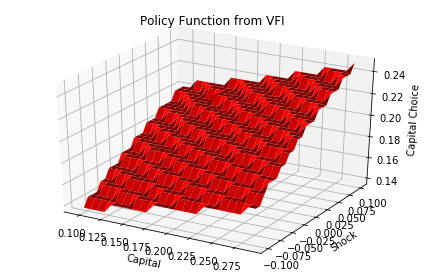
\includegraphics[scale = 0.5]{fig1}
		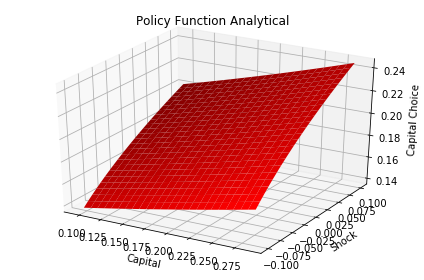
\includegraphics[scale = 0.5]{fig2}
	\end{figure}
	
\end{document}